\section{Equazioni di Hamilton}

\begin{frame}{Hamiltoniana problema 2 corpi ridotto}

\begin{columns}

\begin{column}{0.2\textwidth}

\begin{figure}[!ht]

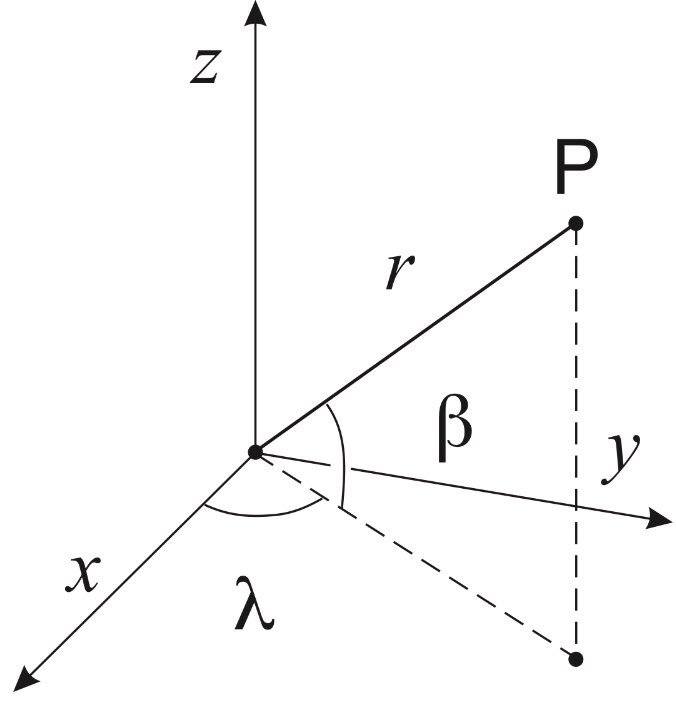
\includegraphics[width=\textwidth]{analytic}

\end{figure}


\end{column}

\begin{column}{0.8\textwidth}

\begin{align*}
&T=\frac{1}{2}\mu(\dot{r}^2+r^2\dot{\beta}^2+r^2\cos{\beta}^2\dot{\lambda}^2)\\
&V=-k^2\frac{\mu}{r}\\
&L=T-V
\end{align*}

\end{column}

\end{columns}

\begin{block}{Momenti coniugati}

\begin{align*}
&p_r=\PDy{\dot{r}}{L}=\mu\dot{r}\\
&p_{\beta}=\PDy{\dot{\beta}}{L}=\mu r^2\dot{\beta}\\
&p_{\lambda}=\PDy{\dot{\lambda}}{L}=\mu r^2\cos{\beta}^2\dot{\lambda}
\end{align*}

\end{block}

\begin{block}{Hamiltoniana}

\begin{align*}
&H(p,q)=\frac{1}{2\mu}(p_r^2+\frac{1}{r^2}p_{\beta}^2+\frac{1}{r^2\cos{\beta}^2}p_{\lambda}^2)-\frac{k^2\mu}{r}
\end{align*}

$\dot{p}_{\lamdba}=0$


\end{block}

\end{frame}


\section{Equazione di Hamilton-Jacobi}



\section{Sistemi integrabili e degenerazione}


